% A Three fold Brochure based on the Latex document class-leaflet

% Brochure created by Joaquim Ignatious Monteiro with inputs from online community
 
\documentclass[notumble,10pt,a4paper]{leaflet} 

% notumble - By default (tumble) the contents of the backside sheet is printed upside down. The option no tumble supresses that.

% Please find the remaining options at http://ctan.math.illinois.edu/macros/latex/contrib/leaflet/leaflet-manual.pdf

\usepackage{color}
\usepackage{flowfram}
\usepackage{graphicx}
\usepackage{wrapfig}
\usepackage{rotating}
%\usepackage{multirow}
%\usepackage{array}
%\usepackage{multirow}
\usepackage{titlesec}
%\usepackage[usenames,dvipsnames]{xcolor}
\usepackage{setspace}    % Adjust line spacing    
\onehalfspacing          % Adjust line spacing  \doublespacing 
\usepackage[inline]{enumitem}

% Agregar español
\usepackage[utf8]{inputenc}
\usepackage[spanish]{babel}

% Incluye Links; pero sin marco
\usepackage[hidelinks]{hyperref}

%Incluir citas a libros *.bib
\usepackage{cite}
\usepackage{url}

%\titleformat*{\subsection}{\color{Blue}}

%FONT Change
%\renewcommand{\familydefault}{cmss} 
%To Draw a horizontal Line
\newcommand{\sectionline}{
  \nointerlineskip \vspace{\baselineskip}
  \hspace{\fill}\rule{0.8\linewidth}{.7pt}\hspace{\fill}
  \par\nointerlineskip \vspace{\baselineskip}
}
%\AddToBackground{2}{\includegraphics[width=29.7cm]{bkf}}
%\AddToBackground{2}{\includegraphics[width=29.7cm]{cmy}}

% To create a border along the top of each page
% To change border color just search on internet for cmyk colour codes and change the values in the brackets after the option cmyk

\vtwotonetop{1cm}{0.6\paperwidth}{[cmyk]{0,.9,1,.6}}{topleft}%
{0.4\paperwidth}{[cmyk]{0,.9,1,.6}}{topright}

% To create a border along the bottom of each page
% To change border color just search on internet for cmyk colour codes and change the values in the brackets after the option cmyk

\vtwotonebottom{1cm}{0.6\paperwidth}{[cmyk]{0,.9,1,.6}}{bottomleft}%
{0.4\paperwidth}{[cmyk]{0,.9,1,.6}}{bottomright}

\begin{document}

% Portada estilizada
\begin{center}
	{\Large Biografía} \\[.3cm]
	\textit{de}\\[.4cm]
	{\huge {Steve Jobs}}\\ [.3cm]
	\textbf{{\large (Exposición grupal)}}\\[.5cm]
	%%\textit{\large{organised by}}
	\vfill
	
	
\includegraphics[width=4cm]{img/logouni.png}\\
	\label{fig:logo}
	\textbf{Universidad Nacional de Ingeniería}\\
	{\large \textbf{Facultad de Ingeniería Mecánica}}\\[.5cm]
	\textit{\large{Escuela profesional de}}\\[.3cm]
	%%\includegraphics[scale=.15]{ICFOSS_logo}\\
	%%\label{fig:ICFOSS_logo}
	{\large \textbf{Ingeniería Mecatrónica}}\\[.5cm]
	\textit{BRC01-B Comunicación y Redacción}\\
	\large{Docente:\\
		Mg. Magali C. Villegas}
	
	\vfill
	Alumnos:\\ 
	\textbf{Victor A. N. Pozo\\
		Sebastian R. Paredes\\
		Jhon K. Mendoza\\
		Bruno D. Nuñez}\\
\end{center}
\thispagestyle{empty} 

%%%%%%%%%%%%%%%%%%%%%%%%%%%%%%%%%%%%%%%%%
\newpage
\section{\large{Steve Paul Jobs}}
Steven Paul Jobs (San Francisco, California, 25 de febrero de 1955-Palo Alto, California, 5 de octubre de 2011), más conocido como Steve Jobs, fue un empresario y magnate de los negocios del sector informático y de la industria del entretenimiento estadounidense. Fue cofundador y presidente ejecutivo de Apple Inc. y máximo accionista individual de The Walt Disney Company\cite{isaacson2011steve}.

\begin{figure}[h!]
	\centering
	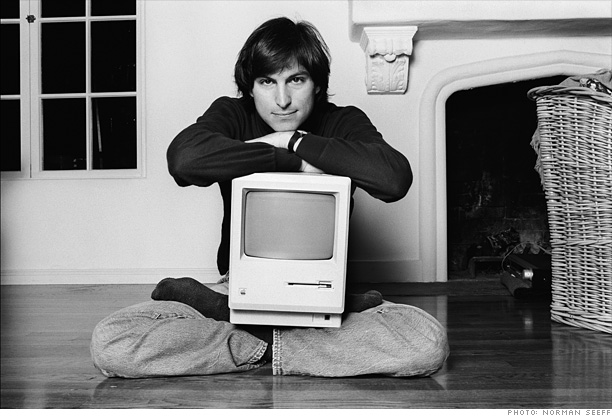
\includegraphics[width=0.9\textwidth]{img/steve-macintosh.jpg}
	\caption{Jobs presentando el macintosh enerode 1984}
\end{figure}

%%%%%%%%%%%%%%%%%%%%%%%%%%%%%%%%%%%%%%
\newpage
\subsection{\large{1976 La fundación de Apple}}
Jobs visita el Homebrew Computer Club de Silicon Valley y decide fundar Apple Computer junto con Wozniak. En aquel pequeño club de aficionados a la informática (su traducción literal sería "Club de los Ordenadores Caseros") los hackers de la época mantenían sus reuniones y charlaban sobre cacharritos.

Jobs y Wozniak enseñaron un día a los socios su Apple I, diseñado y fabricado por Wozniak con material del bricolaje, pero sería la genialidad de Jobs la que les hizo ver que allí había negocio y que podían venderlo en forma de kit para que cualquiera pudiera montarlo en su casa.

Junto con otros amigos y socios capitalistas decidieron fundar una empresa y llamarla Apple Computer. (No sería hasta 2007 que eliminó la palabra computer de su nombre oficial).

\begin{figure}[b]
	\centering
	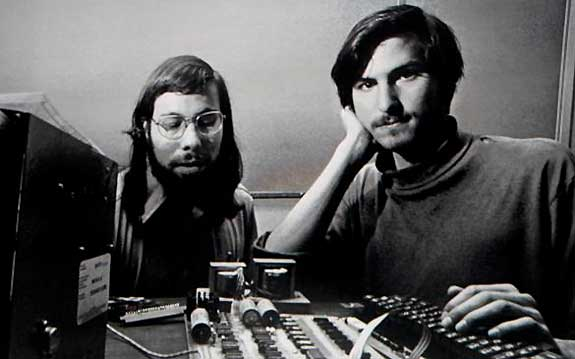
\includegraphics[width=0.9\textwidth]{img/apple.jpg}
	\caption{Jobs y Wozniak}
\end{figure}

%%%%%%%%%%%%%%%%%%%%%%%%%%%%%%%%%%%%%%%%%%%%
\newpage
\subsection{\large{1984 Macintosh}}
Con tan solo 29 años, Steve Jobs vivió el que sería probablemente su momento cumbre desvelando el Macintosh ante la comunidad internacional el 24 de enero de 1984.

Escondido bajo una tela, habló un poco sobre su pequeña nueva criatura para luego enseñarlo dejando que se vieran todas sus posibilidades gráficas e incluso de síntesis de voz.

Era el equipo con el que Jobs había soñado desde que había visto sus componentes en Xerox PARC, la máquina que había diseñado junto a ingenieros como Jeff Rasking, Andy Hertzfeld y otros, siempre en su papel de tirano benevolente – o a veces no tanto, según quienes han trabajado de cerca con él.

\begin{figure}[b]
	\centering
	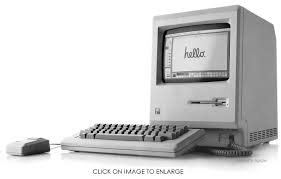
\includegraphics[width=0.9\textwidth]{img/mac.jpeg}
	\caption{Macintosh}
\end{figure}

%%%%%%%%%%%%%%%%%%%%%%%%%%%%%%%%%%%%%%%%%%%
\newpage

\subsection{\large{1995 Toy Story}}
\begin{figure}[b]
	\centering
	
\includegraphics[width=0.9\textwidth]{img/pixar.jpg}
	\caption{Toy Story}
\end{figure}

	La historia de Pixar dice mucho sobre Jobs y su fe en la innovación. Sus comienzos fueron cualquier cosa menos fáciles. Primero, la empresa perdió dinero: cuando en 1985 Jobs fue dejado de lado por Apple, le compró al creador de Star Wars, George Lucas, el pequeño departamento de efectos especiales. En aquel entonces pagó cinco millones de dólares e inyectó otros cinco millones en la compañía, que recibió el nombre de Pixar. 
	En noviembre de 1995 llegó a los cines Toy Story, la primera película animada producida totalmente por computador. Una semana más tarde, Pixar salió triunfalmente a Bolsa. Y Jobs, que poseía un 70 por ciento de la empresa, sumó millones a su cuenta. 
	Cuando Steve Jobs vendió finalmente Pixar a Disney en 2006 por más de 7 000 millones de dólares, la operación pareció más bien una adquisición creativa por parte del socio menor. Pues en aquel momento, la tradicional casa de animación Disney deambulaba sin rumbo tras varios fracasos, y los puestos clave los ocuparon gente de Pixar como el director de Toy Story, John Lasseter. 

%%%%%%%%%%%%%%%%%%%%%%%%%%%%%%%%%%%%%%%%5
\newpage
\subsection{\large{2007 iPhone}}
\begin{figure}[b]
	\centering
	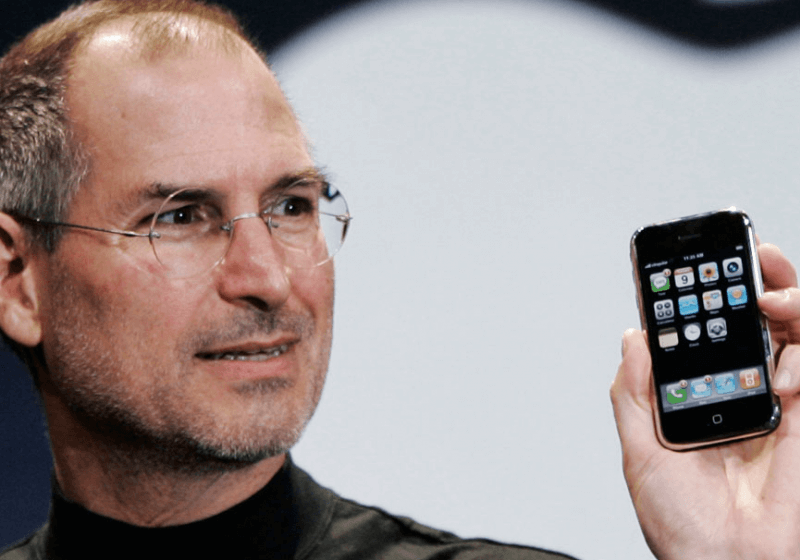
\includegraphics[width=0.9\textwidth]{img/iphone.png}
	\caption{Jobs presentando el iPhone, 2007}
\end{figure}

	Cuando parecía que poco más se podía inventar, Steve Jobs todavía tenía otro as en la manga, pero era tan arriesgado jugarlo que pocos lo anticiparon: suponía remover los cimientos de toda la industria de las comunicaciones actuales.
	Pero en 2007 el cofundador de Apple volvió a enfundarse sus vaqueros, sus zapatillas deportivas y su camiseta negra y lo hizo de nuevo: "Esto es un iPod, un teléfono y un dispositivo con conexión a Internet. Pero no son tres aparatos distintos: son uno solo. Y lo hemos llamado iPhone".

	En 2011 Apple ha señalado que ya ha vendido más de 100 millones de iPhones de los distintos modelos que Steve Jobs ha ido meticulosamente presentando desde entonces. Y probablemente serán todavía muchos más.

%%%%%%%%%%%%%%%%%%%%%%%%%%%%%%%%%%%%%%%%

% bibliografía
% Requiere multiple compilación

%pdflatex	 *.tex
%bibtex		 *.aux  !!! (*.AUX)
%pdflatex	 *.tex

\bibliography{steve-jobs}{}
\bibliographystyle{plain}

\end{document}
